\documentclass[a4paper,10pt]{book}
\usepackage[utf8x]{inputenc}
\usepackage[spanish] {babel}
\usepackage{graphicx} 
\usepackage{array,multirow,tabulary} %Usados para las tablas
\usepackage[left=2cm,top=2cm,right=2cm,bottom=2cm]{geometry} %Definimos los Margenes
\pagestyle{empty}
\usepackage{blindtext}
\usepackage{microtype}
\renewcommand{\familydefault}{\sfdefault}
\newcommand{\Titulo}{Lista de Componentes Pinguino Base}
\newcommand{\Autor}{Alexis A. Sánchez O.}
\newcommand{\Fecha}{Noviembre 2011}
\title{\Titulo}
\author{\Autor}
\date{Noviembre 2011}
\begin{document}
\begin{center}
  Lista de Materiales \\
  Pinguino Base \\
   \Large {Lista de Componentes}\\
   \begin{tabular}{| l | c | c |  c |}
     \hline
      {\bfseries Componente}		& {\bfseries Valor}	& {\bfseries Cantidad} 	& {\bfseries Imagen} \\ \hline
      Microcontrolador PIC		& 18F4550		& 1 			& 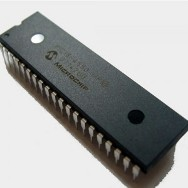
\includegraphics[width=0.125\textwidth]{img/pic-18f4550.jpg} \\ \hline
      Conector USB Tipo B (Hembra)	& 			& 1 			& 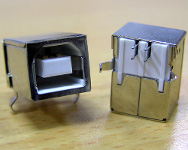
\includegraphics[width=0.125\textwidth]{img/usb-b.jpg} \\ \hline
      SWITCH 2 Estados			& 			& 1 			& 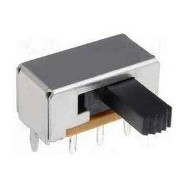
\includegraphics[width=0.125\textwidth]{img/switch-vertical.jpg} \\ \hline
      Pulsador Momentario Omron 	& 			& 1 			& 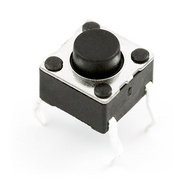
\includegraphics[width=0.125\textwidth]{img/pulsador.jpg} \\ \hline
      Capacitor Electrolitico	 	& 0.33uf/50v		& 1 			& 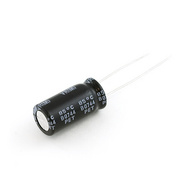
\includegraphics[width=0.125\textwidth]{img/electrolitico.jpg} \\ \hline
      Capacitor Ceramico	 	& 0.1uf			& 3 			& 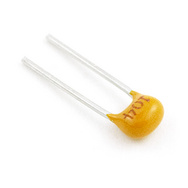
\includegraphics[width=0.125\textwidth]{img/104.jpg} \\ \hline
      Capacitor Ceramico	 	& 22pf			& 2 			& 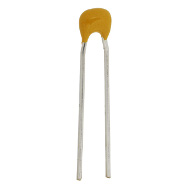
\includegraphics[width=0.125\textwidth]{img/22.jpg} \\ \hline
      Capacitor Electrolitico	 	& 0.22uf/50v		& 1 			& 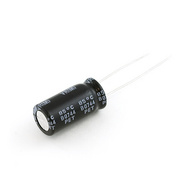
\includegraphics[width=0.125\textwidth]{img/electrolitico.jpg} \\ \hline
      Capacitor Electrolitico	 	& 10uf/50v		& 1 			& 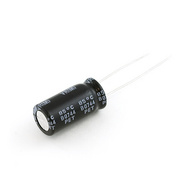
\includegraphics[width=0.125\textwidth]{img/electrolitico.jpg} \\ \hline
      Diodo			 	& 1N4007		& 1 			& 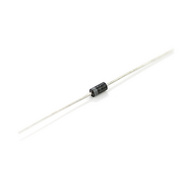
\includegraphics[width=0.125\textwidth]{img/diodo.jpg} \\ \hline   
   \end{tabular}
   \newpage 
   \begin{tabular}{| l | c | c |  c |}
     \hline
      {\bfseries Componente}		& {\bfseries Valor}	& {\bfseries Cantidad} 	& {\bfseries Imagen} \\ \hline  
      Conector Jack para Alimentación	& 			& 1 			& 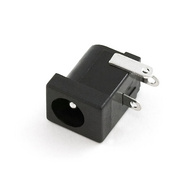
\includegraphics[width=0.125\textwidth]{img/jack.jpg} \\ \hline
      Regulador de Voltaje 5V		& 7805			& 1 			& 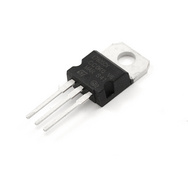
\includegraphics[width=0.125\textwidth]{img/7805.jpg} \\ \hline
      Conector Macho Vertical		& 			& 3 			& 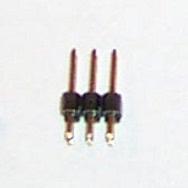
\includegraphics[width=0.125\textwidth]{img/espadin.jpg} \\ \hline
      Conector Macho 90º		& 			& 6 			& 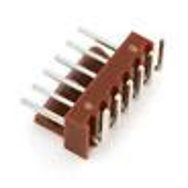
\includegraphics[width=0.125\textwidth]{img/icsp.jpg} \\ \hline
      Conector Header Hembra 8 pines	& 			& 4 			& 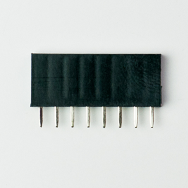
\includegraphics[width=0.125\textwidth]{img/header.png} \\ \hline
      Cristal				& 20Mhz			& 1 			& 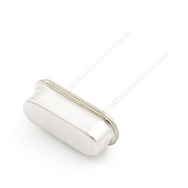
\includegraphics[width=0.125\textwidth]{img/cristal.jpg} \\ \hline
      Resistencia Electrica		& 470 Ohm		& 1 			& 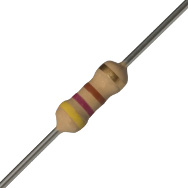
\includegraphics[width=0.125\textwidth]{img/470.jpg} \\ \hline
      Resistencia Electrica		& 10k  Ohm		& 1 			& 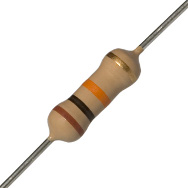
\includegraphics[width=0.125\textwidth]{img/10K.jpg} \\ \hline
      Led 3mm				& 			& 1 			& 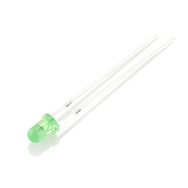
\includegraphics[width=0.125\textwidth]{img/led.jpg} \\ \hline
      Base DIP-40 			& 			& 1 			& 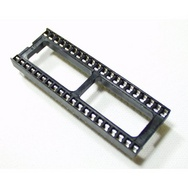
\includegraphics[width=0.125\textwidth]{img/DIP-40.jpg} \\ \hline
   \end{tabular}
 \end{center}

\end{document}
